\section{Experimental protocols and reproducibility}\label{app:protocols}
This appendix gives protocol details for the experiment families in Table~\ref{tab:exp_overview}; their protocol classifications are not changed by the choice of displayed figures. Appendices~\ref{app:year_geometry}--\ref{app:reproduce} contain the historical YearPredictionMSD geometry study, the complete ESS tables and the reproduction assets.

\subsection{Targets, preprocessing and geometry}
German uses the frozen $61$-coordinate encoding without an intercept, prior precision $1$, and a fixed posterior metric. Bank uses reference-level categorical coding, standardized continuous features and an intercept. The $\log(1+\texttt{previous})$ sensitivity replaces and restandardizes only that continuous column; the winsorized version caps it at $22$, the declared $99.9\%$ quantile, affecting $45$ rows. Labels and other design columns are unchanged. The maximum standardized value decreases from approximately $119.1$ to $10.1$ and $12.0$ respectively. Each altered design has its own Gaussian-prior posterior: retaining the same prior form does not make this a posterior-preserving reparameterization.

Fixed-size synthetic logistic targets share $N=30{,}000,d=20$. Three have design covariance condition number $10^4$: correlated signal1, scaled signal1 and correlated signal3. The benign target has design condition number $10$. Measured posterior Hessian condition numbers are approximately $3097,3465,1660,9.65$. These targets differ in more than one posterior characteristic; their comparison does not identify a causal effect of condition number alone. P3B uses the distinct AR(1) mechanism described in the main text, no intercept and prior $N(0,I)$. Its data-generation and label-uniform seeds are $206000$ and $206001$; the coefficient vector and construction are recorded in the frozen configuration.

Constant-metric drift and noise both use the same $P$. Metric regularization is recorded separately from the exact prior contribution and from likelihood Taylor caches. The full-H likelihood cache can be reused when the metric already requires the Hessian; the saved runtime ledger, not an assumed theoretical operation equivalence, determines the reported setup. Identity/diagonal pilot arms are not substitutes for a complete independently validated preconditioning ablation on every logistic target.

\subsection{References and quality gates}\label{app:references}
References are approximate full-data, Metropolis-corrected HMC draws \citep{neal2012hmc}. Separate pools are used to check sensitivity and agreement; correlated HMC draws are not treated as iid bootstrap units. Rank-normalized convergence and bulk/tail ESS are assessed as in \citet{vehtari2021rank}. The principal gates require maximum $\widehat R<1.01$, minimum bulk and tail ESS at least $400$, no recorded divergences, minimum acceptance above $0.5$, and study-specific independent-pool agreement checks.

Original Bank initially fails: maximum $\widehat R$ is $1.0136/1.0144$ and minimum tail ESS $315/389$. An explicit reference-only amendment increases each pool from four chains with $256$ warmup and $1024$ retained draws per chain to $1024$ warmup and $8192$ retained draws. The original target, HMC scheme and quality gates remain unchanged; fresh reference seeds are $182010/182011$. Both longer pools pass, with maximum $\widehat R$ approximately $1.0004$, minimum bulk ESS above $28{,}000$, tail ESS above $13{,}000$, and no divergences. No Bank pilot is ranked before this gate passes.

For P3B, each $N$ has two pools of four chains, $1024$ warmup plus $8192$ retained draws per chain, eight leapfrog steps and warmup-only adaptation. Independent-pool agreement requires maximum mean-MCSE standardized difference below $4$ and relative covariance difference below $0.2$. All sizes pass the original gates. Transformed Bank constructs fresh approved references as well. German's original protocol additionally checks normalized functional MCSE and inter-reference functional disagreement; those original thresholds and reference-only baselines are retained in its configuration. A reference diagnostic pass is necessary for these rankings, not proof of stationarity or exact posterior truth.

\subsection{Metrics and estimator objects}\label{app:metrics}
Let $z=(\theta-\hat\theta)$ expressed in the declared posterior-standardized coordinates, and let $v_j$ be the reference variance of coordinate $j$. For seed $s$ and replica $r$, the ergodic coordinate-variance estimate through the declared checkpoint is $\widehat v_{srj}$. The later relative error is
\begin{equation}\label{eq:exp_relative_variance}
 E_s=\frac1d\sum_{j=1}^d\left\{\frac1R\sum_{r=1}^R
 \left(\frac{\widehat v_{srj}-v_j}{v_j}\right)^2\right\}^{1/2}.
\end{equation}
The P2/P3 variance estimates accumulate steps $1$ through $K$ without discarding a separate burn-in interval. Their error therefore measures finite-horizon, mode-start estimation rather than a post-burn-in stationary variance estimate; the chain ESS summary in Section~\ref{sec:exp_ess} uses a different retained-sample object. The reported error averages seeds; when both reference means must pass, the less favorable reference mean is used for eligibility. The original German criterion instead normalizes variance-functional errors by a frozen reference-calibration standard deviation. Its target $0.1$ and later relative targets $0.5$ or $0.1$ are therefore not equivalent. The cross-phase sensitivity recomputes the relative metric from saved functionals, without changing the original primary decision.

For SW$_2$, finite endpoint and reference clouds are projected onto fixed unit directions and one-dimensional empirical squared transport distances are averaged before taking a square root. Logistic production comparisons use the declared reference samples and projection resolution, with consistent $128$ directions in the later P3B pipeline. This is not full multivariate population $W_2$. Finite-cloud reference-vs-reference discrepancy is retained and not subtracted as if it were a known bias correction. P4 separately computes full equal-weight empirical optimal transport and an analytic Gaussian population distance.

At a common location, raw gradient-noise MSE is $\mathbb E\|\widehat g-g\|^2$. Preconditioned MSE is $\mathbb E\|P^{1/2}(\widehat g-g)\|^2$. In the row-vector implementation, $P=LL^\top$ and the squared norm is computed after right multiplication by $L$. Exact enumeration of centered observation residuals includes the without-replacement finite-population factor
\begin{equation}\label{eq:exp_finite_population}
 \frac{N^2(N-n)}{n(N-1)}\frac1N\sum_{i=1}^N
 \|r_i-\bar r\|^2,
\end{equation}
or the same norm transformed by $L$. Deterministic prior and anchor corrections cancel in conditional noise. Production P1--P3 minibatches are without replacement; this differs from the iid minibatch notation in Section~\ref{sec:method}. P4 deliberately uses iid with-replacement batches as a standalone quadratic check.

\subsection{Search, validation and uncertainty}\label{app:selection}
Original P2 synthetic selection uses $144$ runs, four new seeds and $R=128$. It freezes $h=0.1$ for all three methods in the first, second and fourth regimes; in correlated signal3, CV1 uses $h=0.05$ and CV2/ULA $0.1$. Held-out uses $96$ runs ($4$ targets, $3$ methods, $8$ seeds), $R=512$, minibatch $32$, and checkpoints $128,512,2048,8192$. Thus the strong-signal comparison is of selected configurations, not a same-step isolation. The four primary variance contrasts at $K=2048$ use $19{,}999$ paired-seed bootstrap draws and $98.75\%$ individual Bonferroni-adjusted intervals. Other P2 metrics and checkpoints use exploratory intervals. Original Bank freezes CV1 $h=0.05$, CV2 $0.00625$, and ULA $0.1$ after its own bounded pilot, not synthetic-optimal settings. P1's primary SW$_2$ target, $0.1133721697$, is the frozen reference-only baseline median plus $0.01$.

Optimized log-transformed Bank uses six batch sizes and initial steps $h=c/L_P$, with $c$ in\[\{0.0015625,0.00625,0.025,0.1,0.4,1.6\}.\] One declared refinement round permits at most two extra steps per method/batch. Pilot seeds choose stable non-dominated candidates using warm/cold time and both accuracy measures, at most two per batch and twelve per method. The $24$ candidates are frozen before validation seeds $205200$--$205207$. Validation horizon $4096$ is set by the declared pilot rule rather than extended after viewing validation. Each P3B size follows the corresponding frozen bounded pipeline, with fresh per-size configurations and seed audits; no transfer of a Bank optimum is assumed.

At variance threshold $\varepsilon$, point-attainment time minimizes declared mean cost among eligible configurations/checkpoints satisfying both reference accuracy means and SW$_2\leq0.3$. Supported time instead requires simultaneous upper accuracy bounds to pass. A minimum is conditional on the validated candidate grid; selecting it from validation data can remain optimistic. If only one method reaches the target, report that fact without an infinite or finite speedup. All $41$ thresholds from $0.20$ to $0.60$, in $0.01$ increments, are retained. Adjacent thresholds are strongly dependent, and checkpoint or configuration changes between them can produce nonmonotone speedup ratios.

P3 optimized inference uses $10{,}000$ paired whole-seed bootstrap resamples, preserving all configuration/checkpoint dependence within the resampled seed. Minima are reselected within each bootstrap draw. Not-Reached mass and conditional intervals are retained. Approximate simultaneous accuracy bands cover the declared eligible configuration/checkpoint, two-reference, two-metric family. The log-transformed Bank critical max-statistic is $3.336$. Calibration with eight seed clusters is approximate and conditional on fixed references; per-$N$ bands do not establish a joint across-$N$ coverage guarantee. Point and supported choices can differ: at log-transformed Bank variance threshold $0.2$, warm speedup is $4.723$ for point-attainment and $5.776$ for supported choices. Figure~\ref{fig:thresholds_app} retains the full curve.
\begin{figure}[tb]
\centering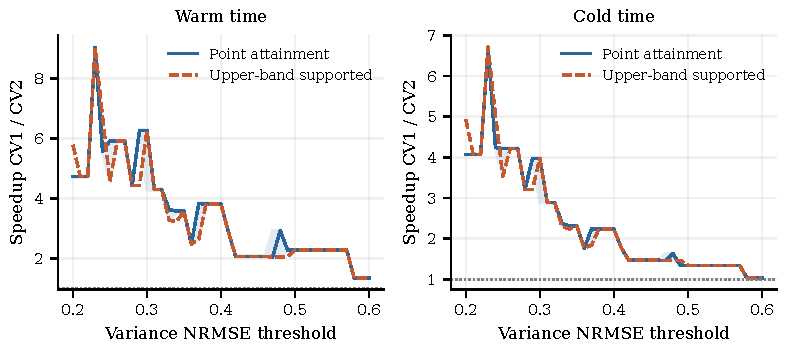
\includegraphics[width=\linewidth]{figures/log1p_thresholds.pdf}
\caption{Complete log-transformed Bank threshold analysis: CV1/CV2 speedup at all $41$ variance-NRMSE thresholds for warm (left) and cold (right) time, under point and supported attainment.}\label{fig:thresholds_app}
\end{figure}

\subsection{Failures and diagnostic side experiments}\label{app:failures}
Nonfinite states or excessive declared standardized radius trigger a numerical failure; a typical frozen radius limit is $100\sqrt d$. Failed replicas are never removed to score a surviving subset. Eligibility follows each original protocol: early P1/P2 comparisons retain valid pre-failure prefixes, whereas optimized P3A/P3B exclude a complete configuration at every checkpoint if any validation seed fails or is incomplete at the full horizon. Retrospectively applying one rule to all phases would change the experiments.

German's twelve diagnostic replays reproduce original streams and $64$ replicas through $2048$. At full-H coefficient $0.8$, CV2 has $14/64$ failures in each seed, beginning at iterations $82$ and $467$; coefficient $0.4$ and paired CV1/ULA controls show no failures in this replay. Independent gradient, Hessian and noise calculations agree to roundoff. The large stochastic-gradient-error drift dominates the tested terminal proposals; this is evidence of a stability limitation at those steps, not an identified implementation bug.

For practical Li2016-style controls \citep{li2016psgld}, zero-initialized raw-gradient RMSprop uses $\alpha=0.99$ and $\epsilon=10^{-5}$ in the detailed German replay, with prior/CV correction excluded from metric accumulation and the adaptive correction term omitted. At coefficient $0.256$, Li-pCV2 has $27/64$ and $33/64$ failures, starting at iteration $3$; paired Li-pCV1 does not fail. Sparse coordinates absent from early minibatches retain $D=1/\epsilon$, while CV2's full-data correction acts in those coordinates. These failures concern this exploratory zero-initialized, correction-omitted implementation and may reflect its design choices rather than a limitation of Li et al.'s method. Adaptive preconditioning is outside the primary comparison because the shared fixed metric controls posterior geometry, not because these runs establish method-level inferiority.


A subsequent bounded initialization sensitivity uses two fresh JAX seeds, $64$ replicas and $2048$ steps on the same German target. It holds $h=1.32\times10^{-5}$, $\alpha=.99$, $\epsilon=10^{-5}$ and batch $32$ fixed, pairing minibatch and Gaussian streams while changing only the initial accumulator. Li-pCV2 records $30/64$ and $29/64$ failures with zero initialization, versus $0/64$ in both runs with an independent $32$-minibatch anchor initializer. The Li-SGLD and Li-pCV1 controls record no failure under either initialization. These are new diagnostic streams, not exact replays of the earlier NumPy failures. They support initialization sensitivity of early stability, without establishing posterior accuracy, mixing or optimized adaptive efficiency; no further adaptive search is used for the primary comparison.

The Bank diagnostic first audits $61$ common states (anchor, reference, trajectory, stress and selected failure states). The high-leverage sensitivity reconstructs all $28$ failed-replica trigger batches, preserving the dependence induced by common seeds. The one other triggering observation is also retained; observation $29182$ is not asserted to cause every failure. Counterfactual replacement does not remove observations from the inference target. The feature-sensitivity stage then changes the target explicitly and uses fresh references and validation seeds.

Intermediate log-transformed Bank tests fix $n=16,h=0.025$ and vary $K\in\{128,256,384,512\}$. Both methods first meet the loose target at $K=256$, giving warm speedup $0.876$ with interval $[0.830,0.913]$, favoring CV1. A post-result threshold sweep finds different rankings at tighter criteria. These fixed-configuration results are preserved rather than replaced by the later optimized positive example. They explain why a common threshold or one favorable configuration is insufficient to determine an optimized frontier.

\subsection{Runtime and scaling decomposition}\label{app:cost}
The Gaussian prior is evaluated exactly once per stochastic-gradient call; its curvature is included once in the full posterior metric. Shared anchor preparation is measured once and attributed to each independently compared ensemble using it. CV1 also pays for full-H metric construction. Component records may aggregate Hessian assembly, inversion and noise factorization; where they do, no unmeasured separate timings are invented. Warm/cold differences reflect actual compilation/cache attribution. In P2, identical synthetic signatures reuse the compilation cache after the first target; later cold timings are not fresh-process costs.

For selected prefixes, let $Q_m=K_mc_m$ denote measured sampling time and $A_m$ the attributed mode/prepare time. The identity
\begin{equation}\label{eq:exp_cost_identity}
 \frac{T_1}{T_2}=\frac{K_1}{K_2}\frac{c_1}{c_2}
 \frac{1+A_1/Q_1}{1+A_2/Q_2}
\end{equation}
is bookkeeping, not a fitted model. The P3B supplement checks $87$ unique selected prefixes, $696$ seed-prefix records, $656$ decomposition identities and $164$ endpoint identities. Timing is per batched $512$-replica update, not serial single-chain cost.

At variance threshold $0.4$, CV1 changes batch $32\to16$ between endpoint dataset sizes. At $0.3$, it changes $(n,h,K)=(16,0.05,512)$ to $(16,0.1,384)$, while CV2 remains at $n=1,K=256$. At $0.2$, CV1 trades batch $16\to32$ for steps $2048\to1024$; CV2 remains at $n=1,K=1024$. These changes, plus shared setup dilution, explain why raw gradient-noise rates do not determine speedup alone. At the loose target, the best CV2 choices already sit on the tested minimum batch and earliest checkpoint; further variance reduction cannot necessarily save work within that grid. Figure~\ref{fig:cost_app} shows recorded components; because selected batches differ across accuracy targets and $N$, component differences are not pure per-step algorithmic overhead. Removing setup is a sensitivity analysis, not a replacement official ranking. Correction-only microbenchmark timings were not saved.
\begin{figure}[tb]
\centering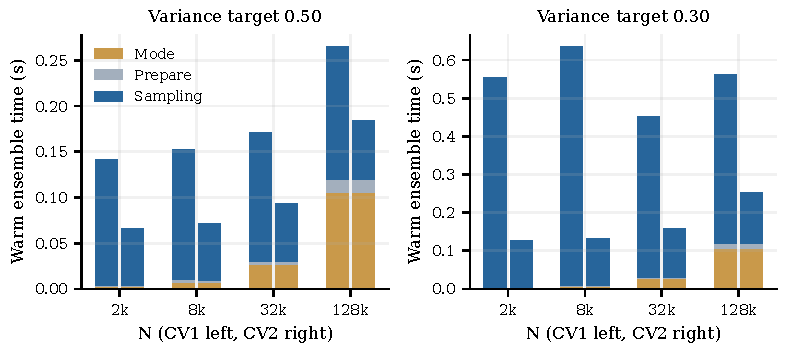
\includegraphics[width=\linewidth]{figures/cost_components.pdf}
\caption{Mode, preparation and sampling components of setup-inclusive warm time for the selected P3B configurations at variance targets $0.5$ (left) and $0.3$ (right); within each $N$, CV1 is left and CV2 right.}\label{fig:cost_app}
\end{figure}

\FloatBarrier
\subsection{Per-size validated accuracy--cost frontiers}\label{app:n_frontiers}
Figure~\ref{fig:n_frontiers_app} retains all $168$ eligible configuration/checkpoint points per synthetic dataset size, with separate SW$_2$--time and variance--time boundaries. The same non-dominance and full-horizon eligibility rules apply as for transformed Bank. Times include setup; errors use the worse reference mean, with common axis limits across sizes. Marginal boundaries can select different configurations and do not establish joint attainment. The main-text speedups impose both requirements through~\eqref{eq:exp_joint_time}. All optima are grid-restricted and subject to validation-selection optimism. Cold costs and supported choices remain in the full analysis.
\begin{figure}[p]
\centering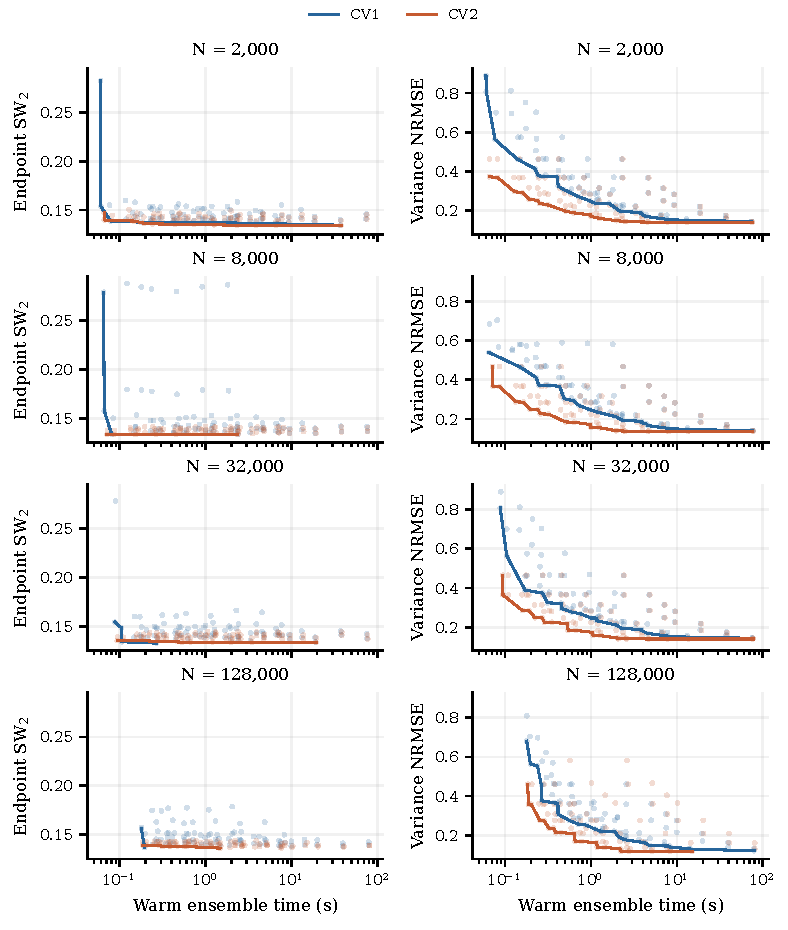
\includegraphics[width=\linewidth,height=0.78\textheight,keepaspectratio]{figures/p3b_full_frontiers.pdf}
\caption{Marginal accuracy--cost comparisons for P3B at $N=2000,8000,32000,128000$ (rows): endpoint whitened SW$_2$ (left) and relative variance NRMSE (right) against setup-inclusive warm time. Faint points are all eligible configuration/checkpoints and lines the non-dominated boundaries; axes are common across sizes.}\label{fig:n_frontiers_app}
\end{figure}
\FloatBarrier
\subsection{Gaussian verification details}\label{app:gaussian}
The tridiagonal-covariance Gaussian target is realized as a finite quadratic sum with heterogeneous rank-one observation Hessians. The actual precision $Q=X^\top X+\lambda_0 I$ and linear term $b=X^\top y$ define the exact posterior $N(Q^{-1}b,Q^{-1})$. The exact mode is supplied through a recorded dense solve, not a hidden optimizer. CV2 is compared against an independent cached quadratic full-gradient oracle, while its own kernel explicitly evaluates the sampled remainder. Batch size is $16$, iid with replacement; checkpoints are $0,16,64,256,1024$, and sampler seeds are $207100$--$207103$.

With $P=I$ or $Q^{-1}$ and $hL_P=0.1$, the finite-step covariance follows the exact Gaussian transition law. Gradient and whitened path discrepancy gates are $10^{-10}$ and $10^{-8}$; a deliberately conservative empirical covariance-to-finite-law check uses Frobenius error divided by $\sqrt d$ at most $0.5$. Observed maximum is $0.1731$. Raw CV2 gradient MSE is $1.469\times10^{-29}$ at $\kappa=10$ and $1.378\times10^{-24}$ at $10^4$, numerical roundoff rather than material stochastic variance. Figure~\ref{fig:gaussian_app} shows analytic transport and covariance error, including stationary discretization bias.
\begin{figure}[tb]
\centering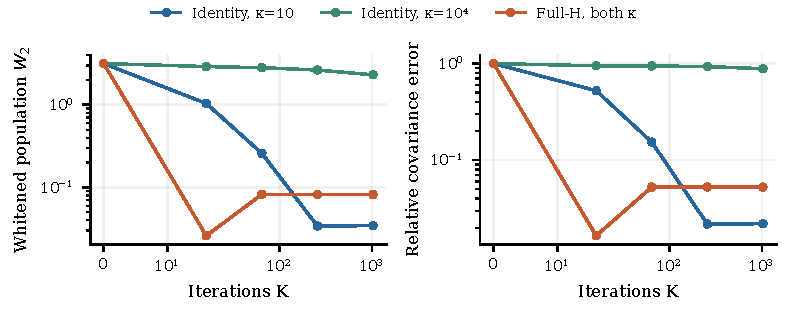
\includegraphics[width=\linewidth]{figures/gaussian_law.pdf}
\caption{Exact Gaussian transport and covariance under the common stability-coefficient rule. Full-H curves coincide across condition numbers; finite-step discretization bias remains.}\label{fig:gaussian_app}
\end{figure}

Empirical full $W_2$ uses exact equal-weight assignment between $512$ endpoints and $512$ independent exact draws, with an independent exact-vs-exact comparison retained as a finite-cloud baseline. It is neither a Gaussian fit nor a sliced approximation. Analytic and empirical distances are reported separately, in original and whitened coordinates. Verification timings include measured setup and shared pre-generated random-input construction; transfer of inputs into JAX is synchronized before timing but not separately attributed. ULA's cached quadratic oracle and CV2's explicit remainder are deliberately different verification workloads, not a production speed comparison.
